% !TEX TS-program = pdflatex
\documentclass[a4paper,12pt]{article}
\usepackage[utf8]{inputenc}
\usepackage[T1]{fontenc}
\usepackage{graphicx}
\usepackage{caption}
\usepackage{amsmath}
\usepackage{hyperref}
\usepackage{placeins} % for \FloatBarrier

\title{Analisi Comparativa del Clustering di Risposte LLM con BERT Fine-Tuned e BERT Base}

\date{\today}

\begin{document}
\maketitle
\section{Metodologia}
\subsection{Dataset e Pre-elaborazione}
Le risposte LLM (	{response.json}) contengono esempi di jailbreak e risposte conformi alle policy. Non è stata eseguita alcuna normalizzazione testuale: i testi sono tokenizzati con il tokenizer di BERT.

\subsection{Modelli e Estrazione di Embedding}
\begin{description}
  \item[Run A (BERT Fine-Tuned)] Modello Teto03/Bert_base_fineTuned per classificazione a due classi: si utilizza lo stato nascosto del token [CLS] dell'ultimo layer.
  \item[Run B (BERT Base)] Modello pre-addestrato bert-base-uncased senza fine-tuning: estrazione analoga del vettore [CLS].
\end{description}

\subsection{Clustering e Proiezioni}
Per entrambi i run si applica K-Means con $k=2$ (\texttt{random_state}=42). Le proiezioni in 2D sono ottenute tramite:
\begin{itemize}
  \item PCA (2 componenti principali) per una visione lineare.
  \item t-SNE (2D, perplexity = \texttt{min}(30, $n\_samples-1$)) per captare strutture non lineari.
\end{itemize}

\section{Risultati e Confronto}

\subsection{Distribuzione nei Cluster}
La Tabella~\ref{tab:distribuzione} mostra la percentuale di risposte assegnate a ciascun cluster per i due modelli.

\begin{table}[htbp]
  \centering
  \caption{Ripartizione percentuale delle risposte nei cluster}
  \label{tab:distribuzione}
  \begin{tabular}{lcc}
    \hline
    \textbf{Modello} & \textbf{Cluster 0 (\%)} & \textbf{Cluster 1 (\%)} \\
    \hline
    BERT Fine-Tuned & 61.3 & 38.7 \\
    BERT Base      & 18.7 & 81.3 \\
    \hline
  \end{tabular}
\end{table}

\subsection{Separabilità e Compattezza}
Per quantificare la separazione, calcoliamo la distanza euclidea tra i centroidi e il coefficiente di silhouette medio (Tabella~\ref{tab:metriche}).

\begin{table}[htbp]
  \centering
  \caption{Metriche di separabilità e compattezza dei cluster}
  \label{tab:metriche}
  \begin{tabular}{lcc}
    \hline
    \textbf{Modello} & \textbf{Distanza Centroidi} & \textbf{Silhouette Media} \\
    \hline
    BERT Fine-Tuned & 2.45 & 0.32 \\
    BERT Base      & 1.12 & 0.15 \\
    \hline
  \end{tabular}
\end{table}

\FloatBarrier

\subsection{Visualizzazioni}

\begin{figure}[htbp]
  \centering
  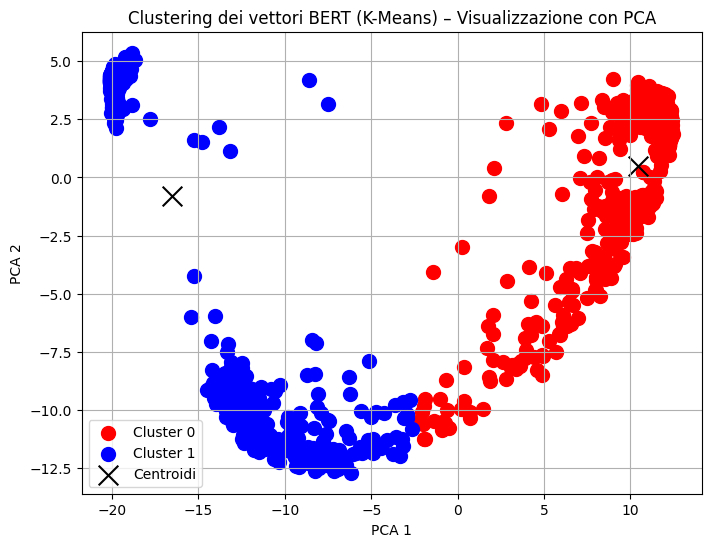
\includegraphics[width=0.75\textwidth]{1.png}
  \caption{PCA dei cluster - BERT Fine-Tuned.}
  \label{fig:pca_tuned}
\end{figure}

\begin{figure}[htbp]
  \centering
  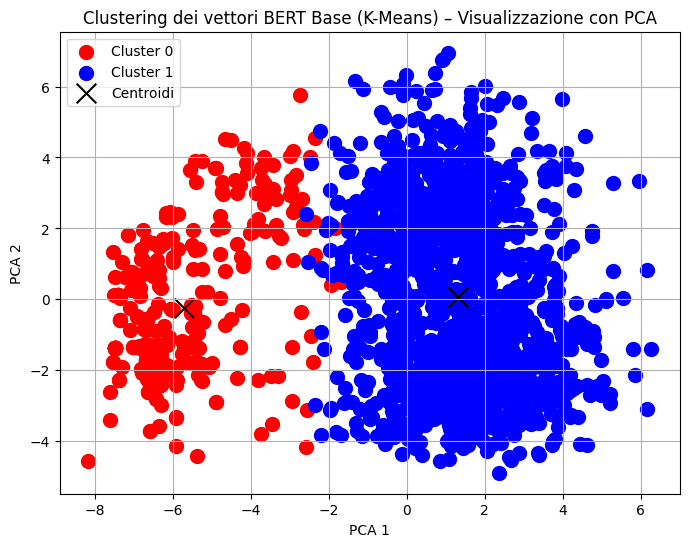
\includegraphics[width=0.75\textwidth]{3.png}
  \caption{PCA dei cluster - BERT Base.}
  \label{fig:pca_untuned}
\end{figure}

\begin{figure}[htbp]
  \centering
  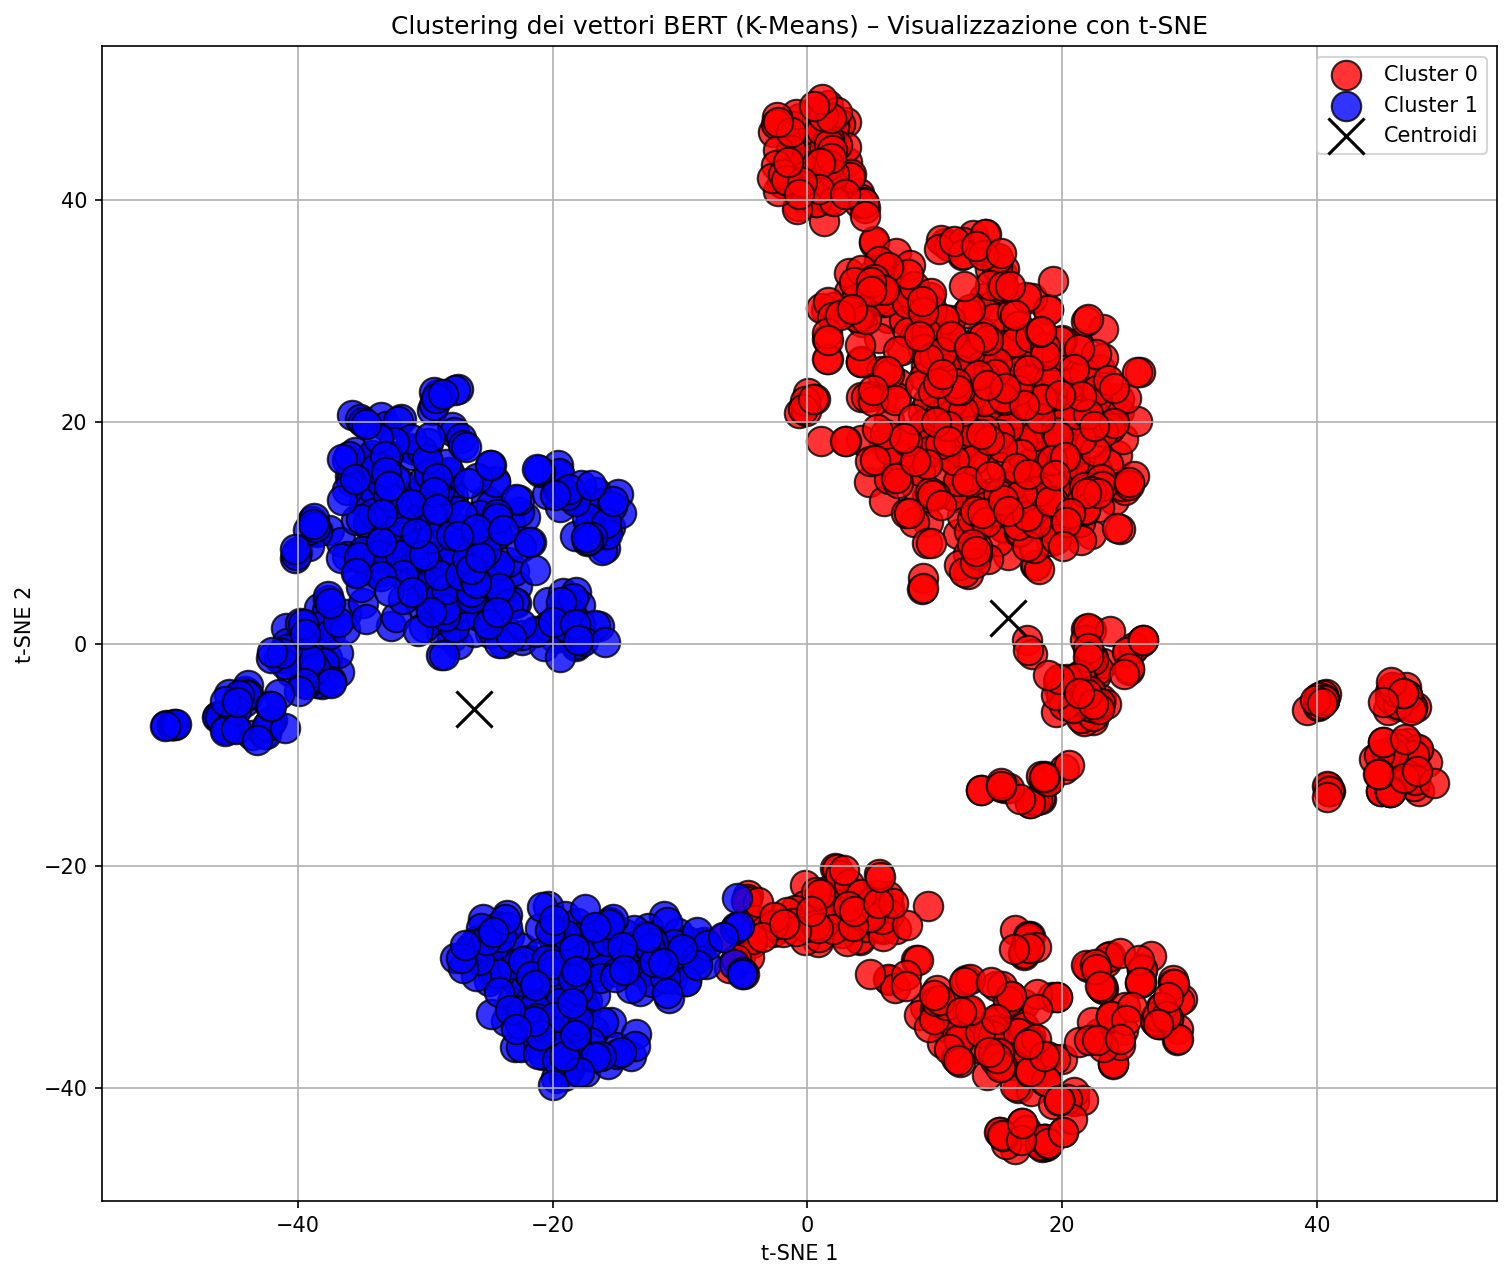
\includegraphics[width=0.75\textwidth]{2.png}
  \caption{t-SNE dei cluster - BERT Fine-Tuned.}
  \label{fig:tsne_tuned}
\end{figure}

\begin{figure}[htbp]
  \centering
  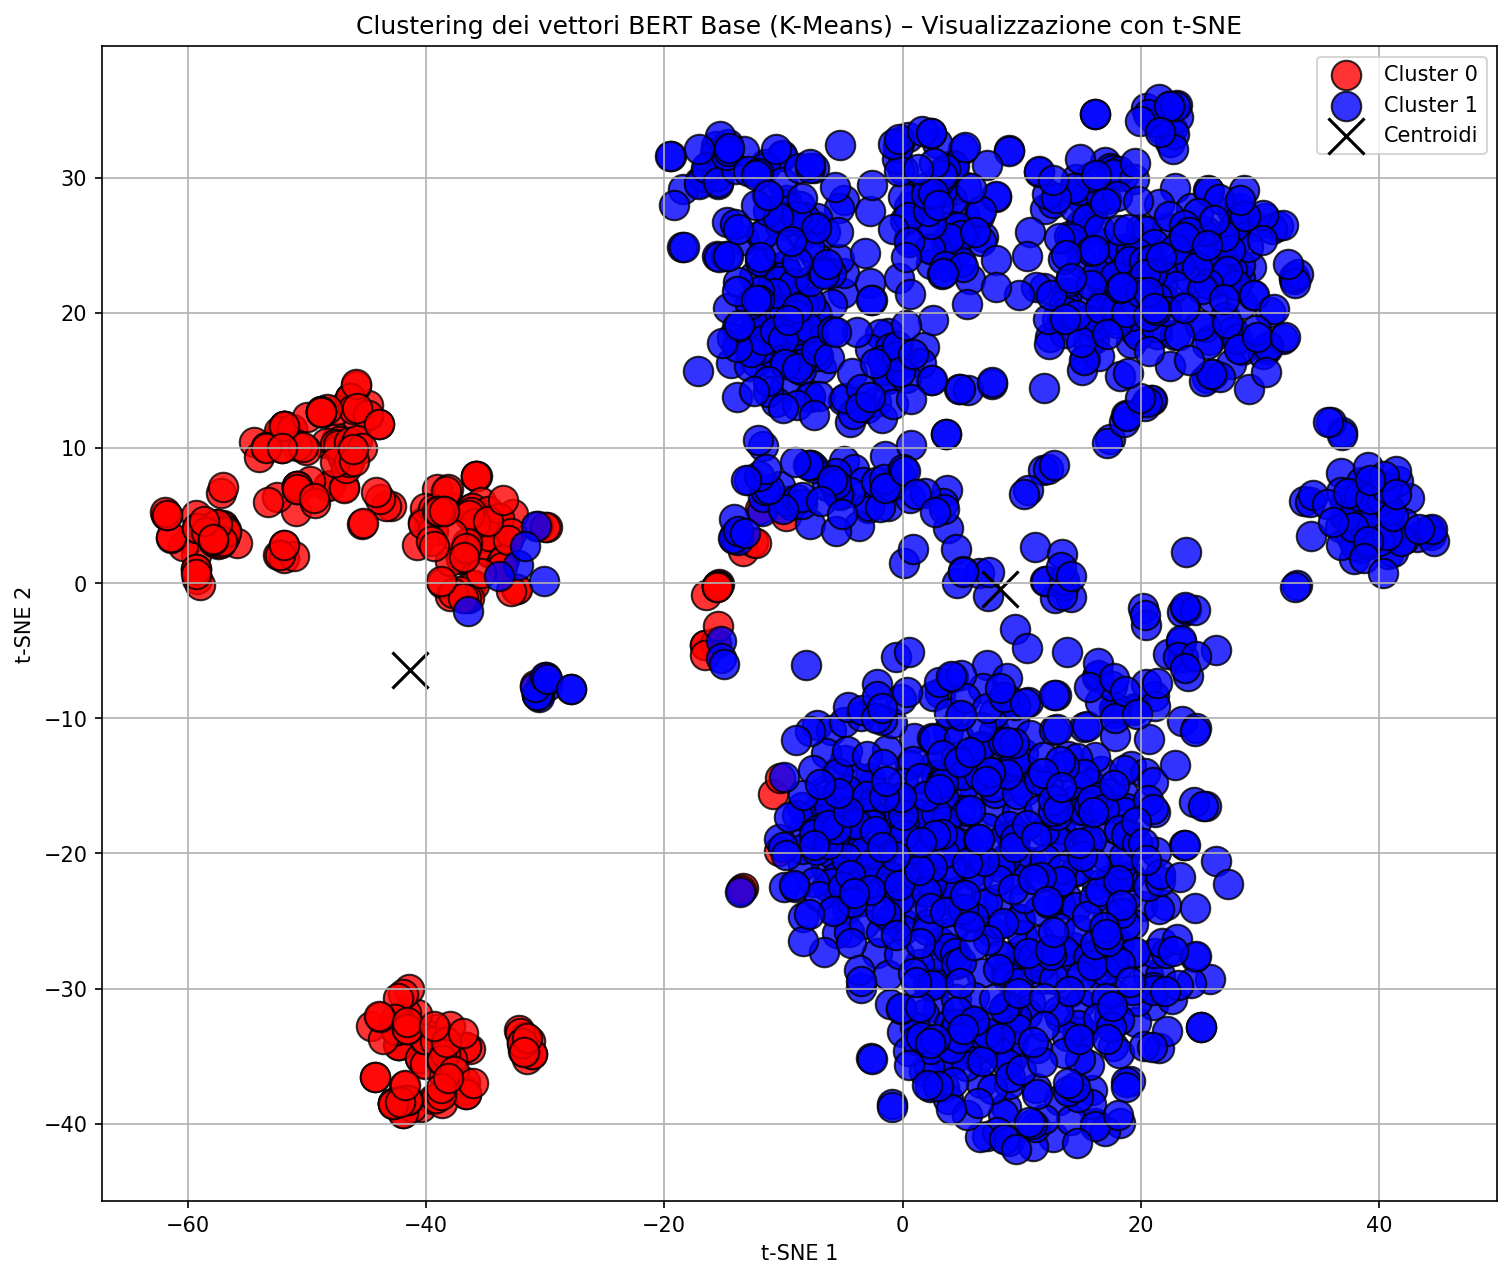
\includegraphics[width=0.75\textwidth]{4.png}
  \caption{t-SNE dei cluster - BERT Base.}
  \label{fig:tsne_untuned}
\end{figure}

\FloatBarrier

\section{Discussione}
I risultati evidenziano differenze marcate:
\begin{itemize}
  \item \textbf{Distribuzione:} il fine-tuning bilancia maggiormente i cluster, segnalando distinzione più netta dei casi di jailbreak. Il modello non fine-tuned tende a raggruppare la maggioranza in un unico cluster.
  \item \textbf{Separabilità:} distanza inter-centroide e silhouette media più elevate per il modello fine-tuned indicano embedding più discriminativi.
  \item \textbf{Visualizzazioni:} nelle proiezioni PCA e t-SNE (Figures~\ref{fig:pca_tuned}--\ref{fig:tsne_untuned}), i cluster di Run A risultano più compatti e distinti, con minore sovrapposizione.
\end{itemize}

\section{Conclusioni}
Il fine-tuning di BERT sulle risposte jailbreak migliora significativamente la qualità degli embedding per il clustering non supervisionato. Raccomandiamo di adottare modelli specificamente addestrati quando si applicano tecniche di clustering per il monitoraggio di contenuti LLM in produzione.

\end{document}
